
\section{\rnn{} assessment vs cut-based triggers}%
\label{sec:off_ana}

This section presents a more detailed assessment of the \rnn{}'s behavior 
in the period 2017--2018 relative to the previous electron trigger's cut-based strategy. 
The potential biases due to introduction of the \rnn into the electron trigger sequence are evaluated in 2017 data events selected using the $Z\rightarrow e^+e^-$ tag-and-probe method~\cite{TRIG-2018-05}.
Since each \tnp{} event has one electron (referred to as the ‘probe electron’) which was not 
used to select that event at trigger level, two analyses were performed to assess the
trigger performance with and without the \rnn{}, with the selection applied either to
the tag electron (Homogeneity Tests) or to the probe electron (Quadrant Analysis). 



The Quadrant Analysis allows a direct assessment of possible bias due to the
introduction of the \rnn{}, when applied to the probe electron, by comparing the profiles for all possible disjoint
decisions from the two trigger classifiers. 

Although it is reasonable to assume that the tag and probe showers 
develop independently, and that the \rnn{} when applied to
the tag selection cannot, in principle, alter the profile of the probes besides
changing the number of \tnp{} pairs, this assumption should be tested. 
An evaluation of any possible systematic effect due to using the \rnn{}, applied to the tag selection, 
in obtaining the likelihood probability distribution functions (PDFs), 
used for offline and final HLT selection, is performed with the Homogeneity Tests.



\subsection{Quadrant Analysis}\label{ssec:quadrant}

The Quadrant Analysis was developed to compare the decisions of two classifiers. Given signal candidates and two classifiers, these are the possibilities:\ either both accept or reject the candidates, or only one accepts the candidates. The four possible decision quadrants are evaluated from shower-shape distributions. Furthermore, in this analysis, it is also possible to evaluate the disagreement between two classifiers. The disagreement between two classifiers $\textbf{A}$ and $\textbf{B}$ can be defined as:

\begin{equation}
    \text{disagreement} = \frac{N_{\textbf{A}}+N_{\textbf{B}}}{N_{\textbf{A}}+N_{\textbf{B}}+N_{\textbf{AB}}+N_{!\textbf{AB}}}
    \label{eq:disagreement}
\end{equation}
where $N_{\textbf{A}}$ ($N_{\textbf{B}}$) is the total number of candidates accepted exclusively by classifier $\textbf{A}$ ($\textbf{B}$) and $N_{\textbf{AB}}$ ($N_{\textbf{!AB}}$) is the total number of candidates accepted (rejected) by both classifiers.

In this approach, only probe electron candidates selected using the $Z\rightarrow e^+e^-$ \tnp method in collision data and an offline selection requirement equivalent with the trigger working point used as classifier are considered. Results in Section~\ref{top:quadrant_results} show
trigger selection performance using the \enquote{tight} requirement for the duplicated triggers during 2017.

\subsubsection{Results}\label{top:quadrant_results}

The Quadrant Analysis was performed on the four shower shapes variables (\reta{}, \rphi{}, \eratio{} and \rhad{})~\cite{TRIG-2018-05} used in the likelihood~\cite{PERF-2017-01} selection, which have the best discrimination power for electrons. 

As shown in Figure~\ref{fig:quadrant_calo_variables_30GeV}, the disagreement is small and in most cases. Here, only the results for $0.6<|\eta|<0.8$ and $35<\ET<40$~\GeV are shown, but this behaviour is also observed for other regions of the $\eteta$ phase space. 
One should note that the working points of the two triggers are not exactly the same, although the \rnn{} aims to achieve the same signal efficiency as the cut-based strategy and was operating as desired.  In other words, the height differences between the blue and red profiles in Figure~\ref{fig:quadrant_calo_variables_30GeV} are mainly due to small efficiency differences between the two triggers.




The two triggers behave very similarly for all variables in the region shown in Figure~\ref{fig:quadrant_calo_variables_30GeV}, even if some slight shifts between blue and red profiles can be seen. This is the case for \reta{} and \rphi{}, where the \rnn{} trigger consistently selects slightly more events in the signal region, i.e.\ ones with slightly narrower showers in $\eta{}$ and $\phi{}$, respectively, in the EM2 layer. The \rnn{} trigger's behaviour shows an even smaller effect in \rhad{}, where tighter tails are observed.%, resulting in fewer electrons with 10\% to 30\% of their energy in EM1, 1\% to 2\% in EM3 and more than 4~GeV hadronic leakage. 
The \eratio{} variable also shows the \rnn{} trigger has a slight bias towards selecting more events in the tail region. 
%Interestingly, a few events with $0.5<\eratio{}<0.7$ are accepted by the trigger with the \rnn{}, probably due to electrons resulting from premature showers with a barycentre near the boundary between two cells in EM1. 
Although similar behaviour is seen in other 
regions of the $\eteta$ phase space.


\begin{figure}[h!]
\centering
\begin{subfigure}[c]{.49\textwidth}
\centering
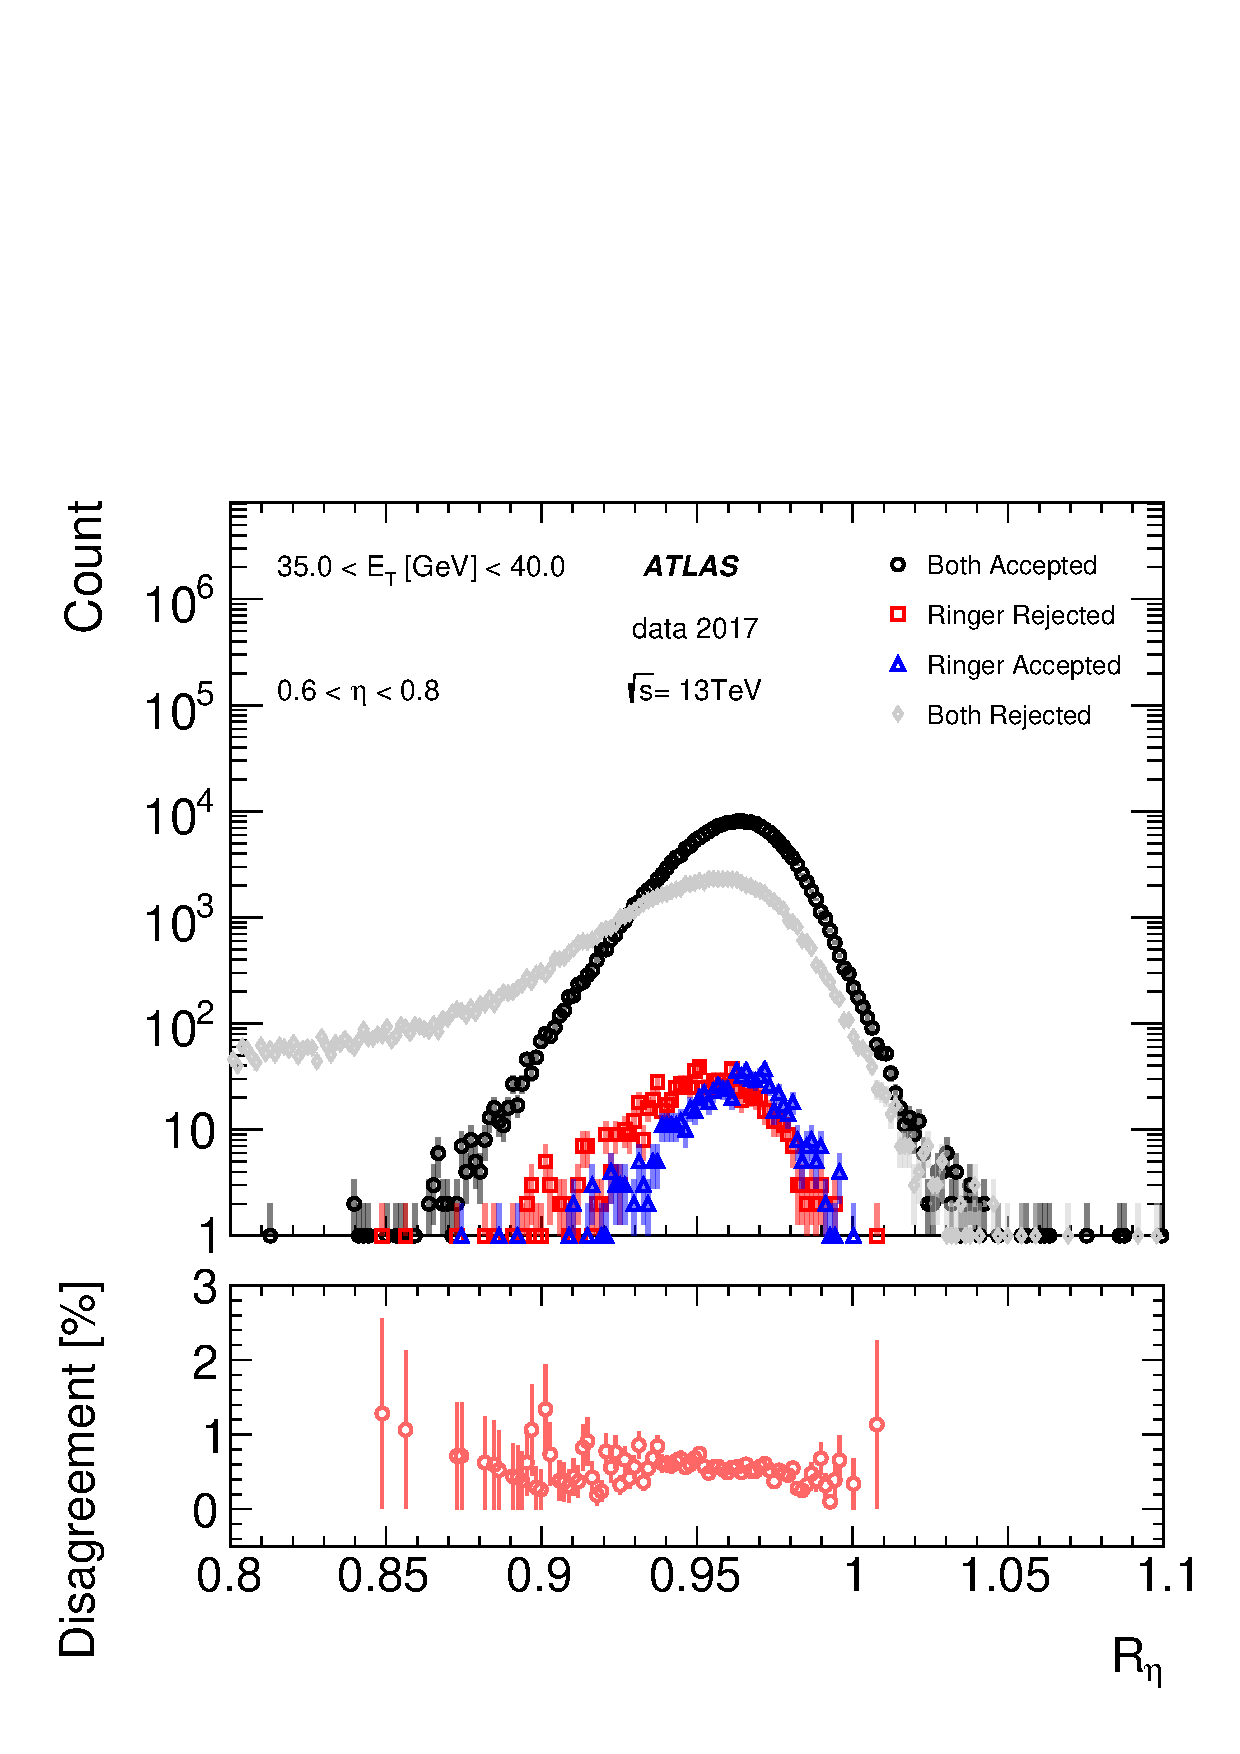
\includegraphics[width=\textwidth]{sections/05_analysis/figures/quadrant_plots/reta.pdf}
\caption{}
\label{fig:quadrant_calo_variables_30GeV_eta}
\end{subfigure}
%\hfill
\begin{subfigure}[c]{.49\textwidth}
\centering
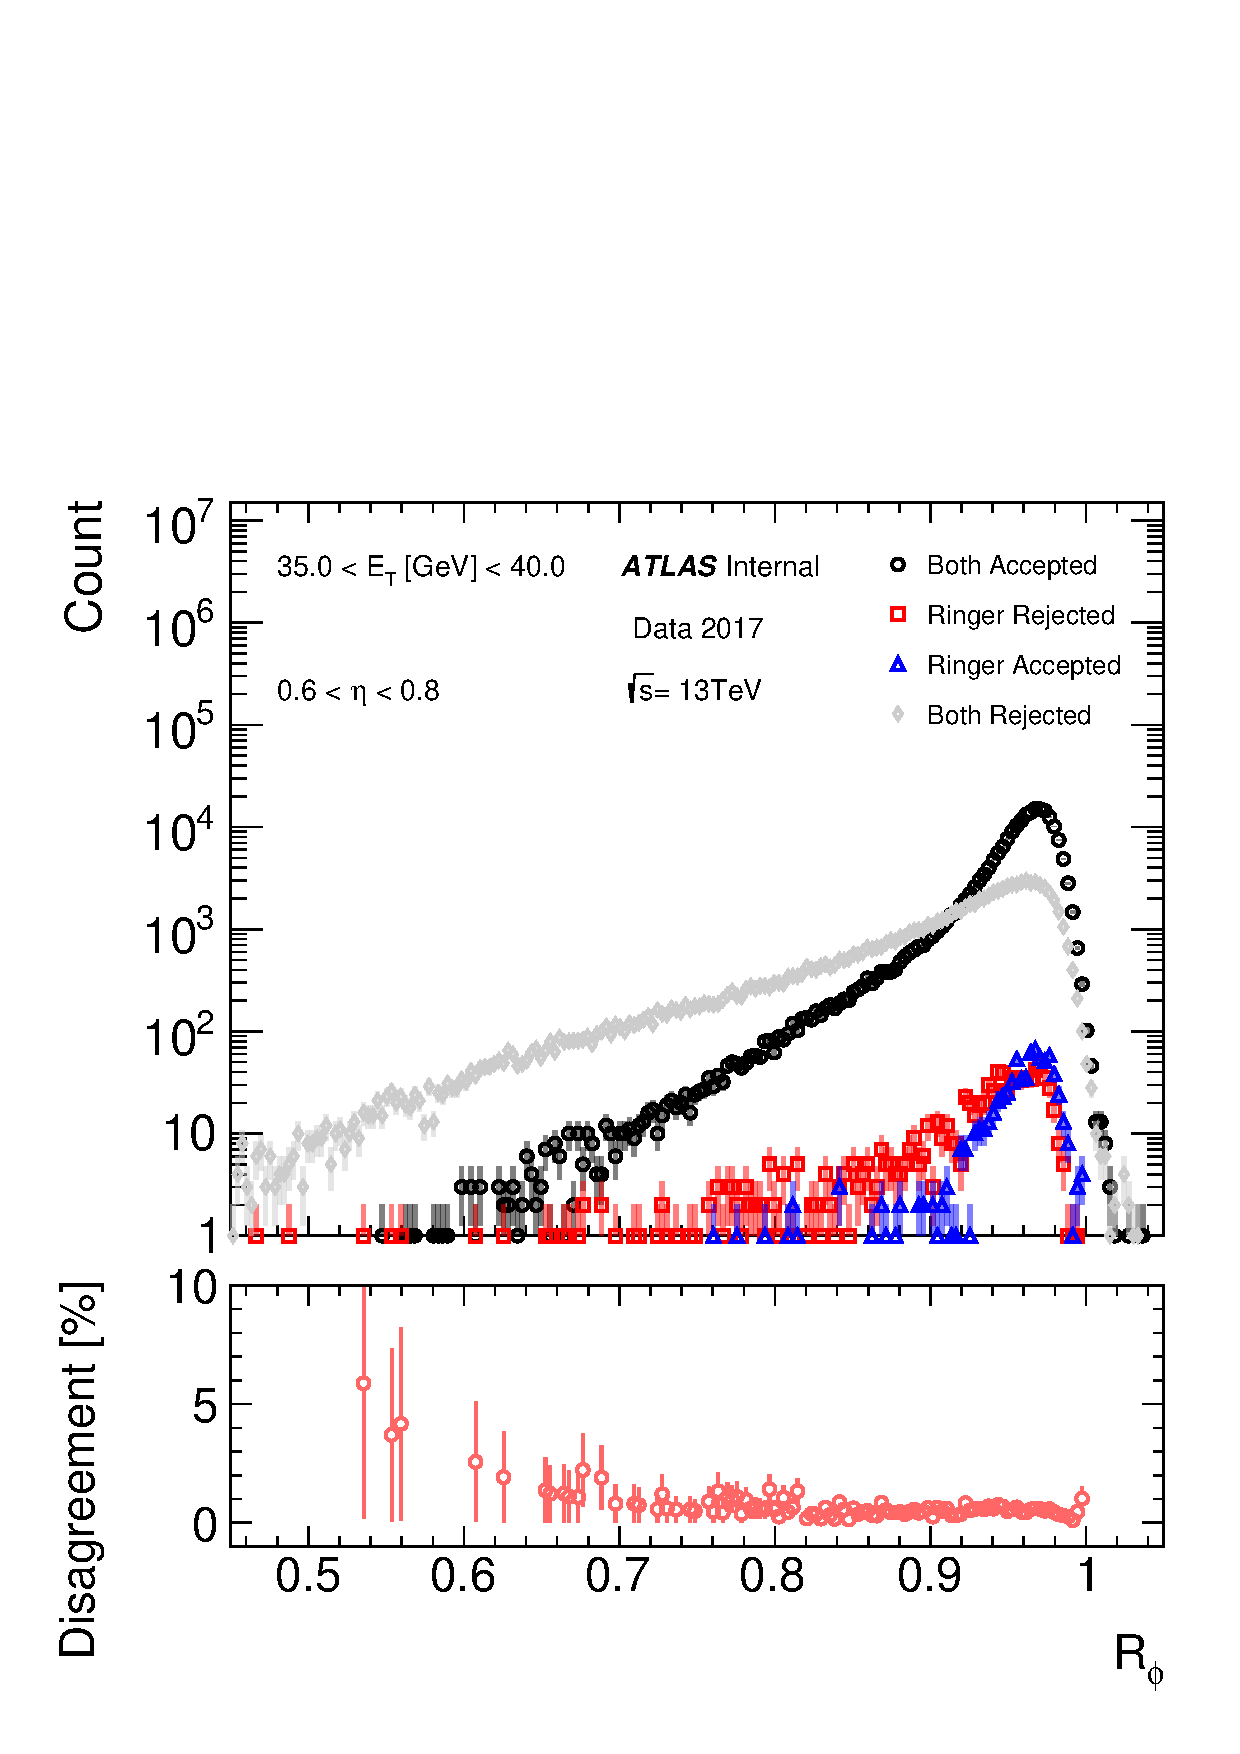
\includegraphics[width=\textwidth]{sections/05_analysis/figures/quadrant_plots/rphi.pdf}
\caption{}
\end{subfigure} 
%\end{figure}
%\begin{figure}[p]\ContinuedFloat
\begin{subfigure}[c]{.49\textwidth}
\centering
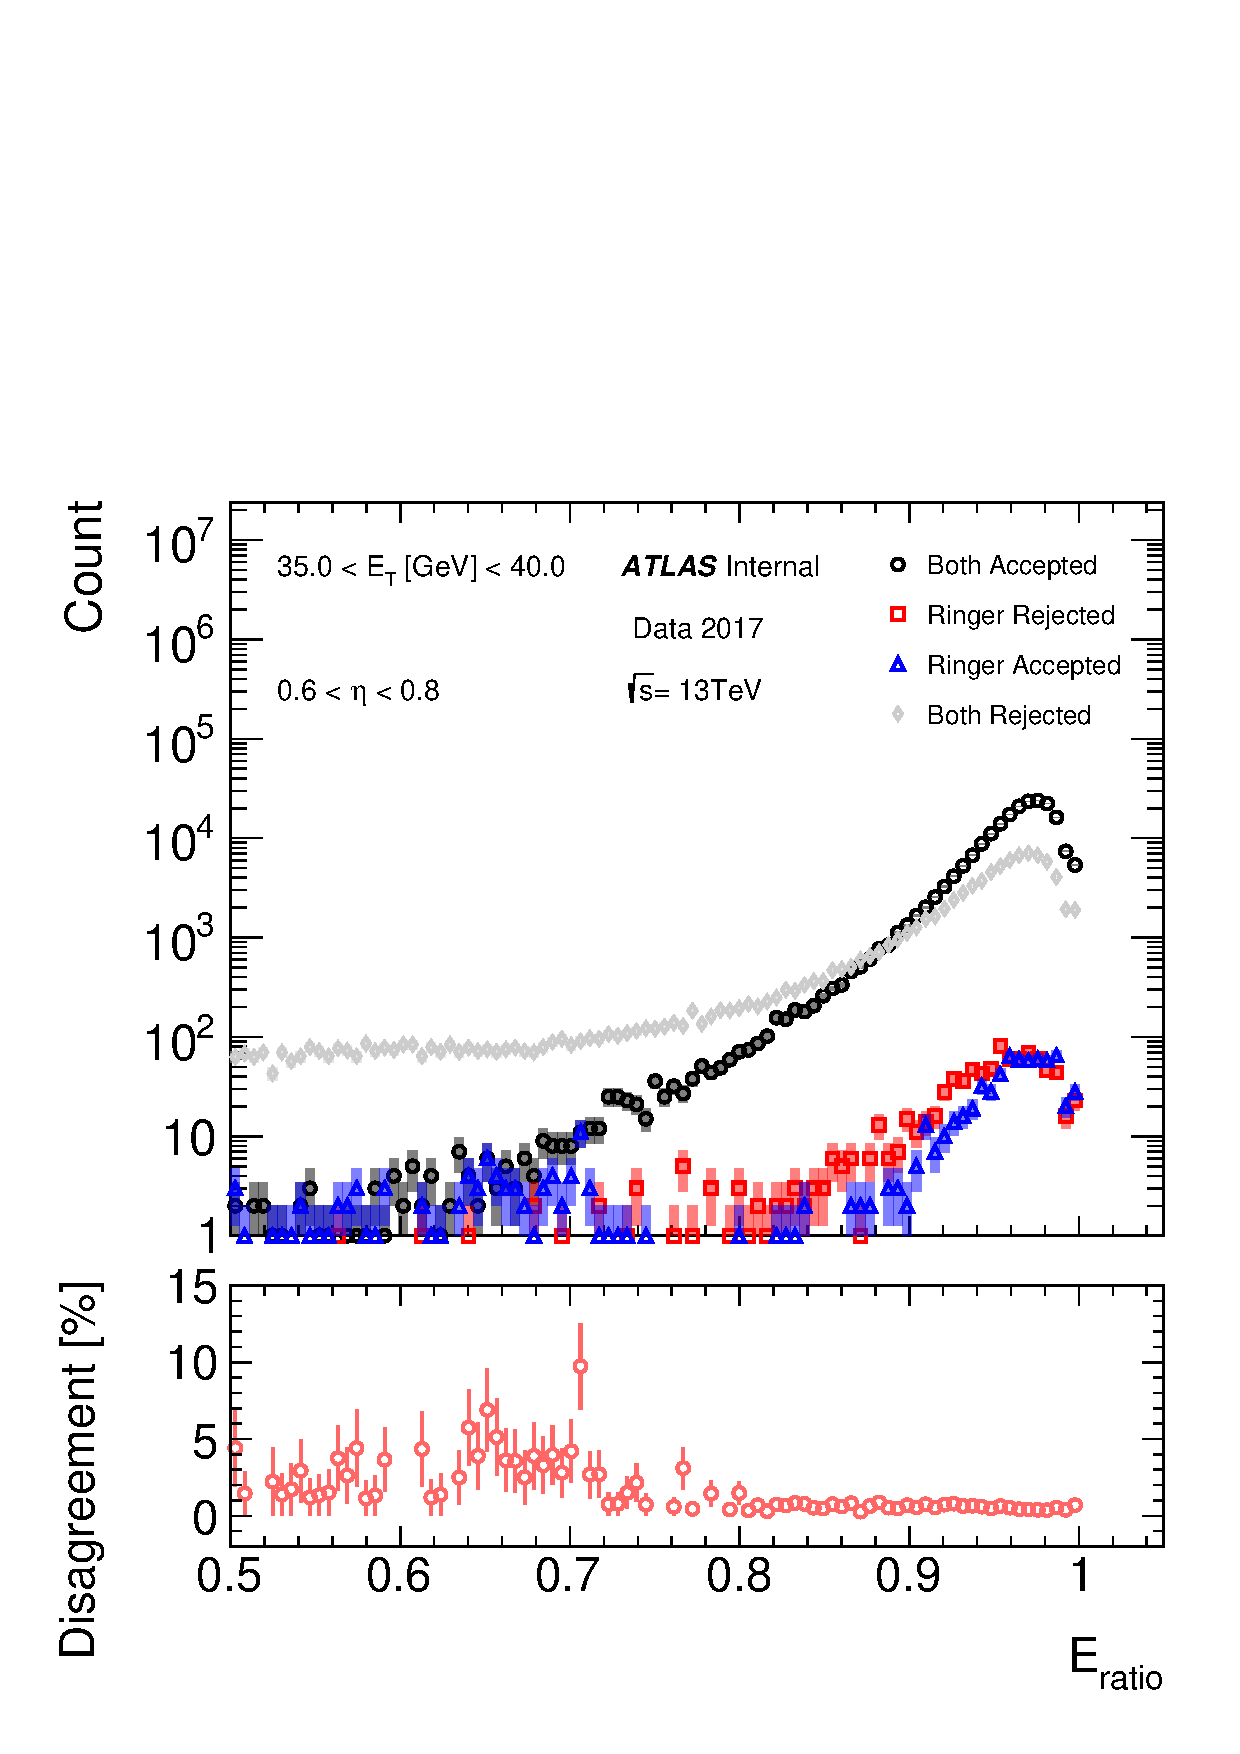
\includegraphics[width=\textwidth]{sections/05_analysis/figures/quadrant_plots/eratio.pdf}
\caption{}
\end{subfigure}
\hfill
\begin{subfigure}[c]{.49\textwidth}
\centering
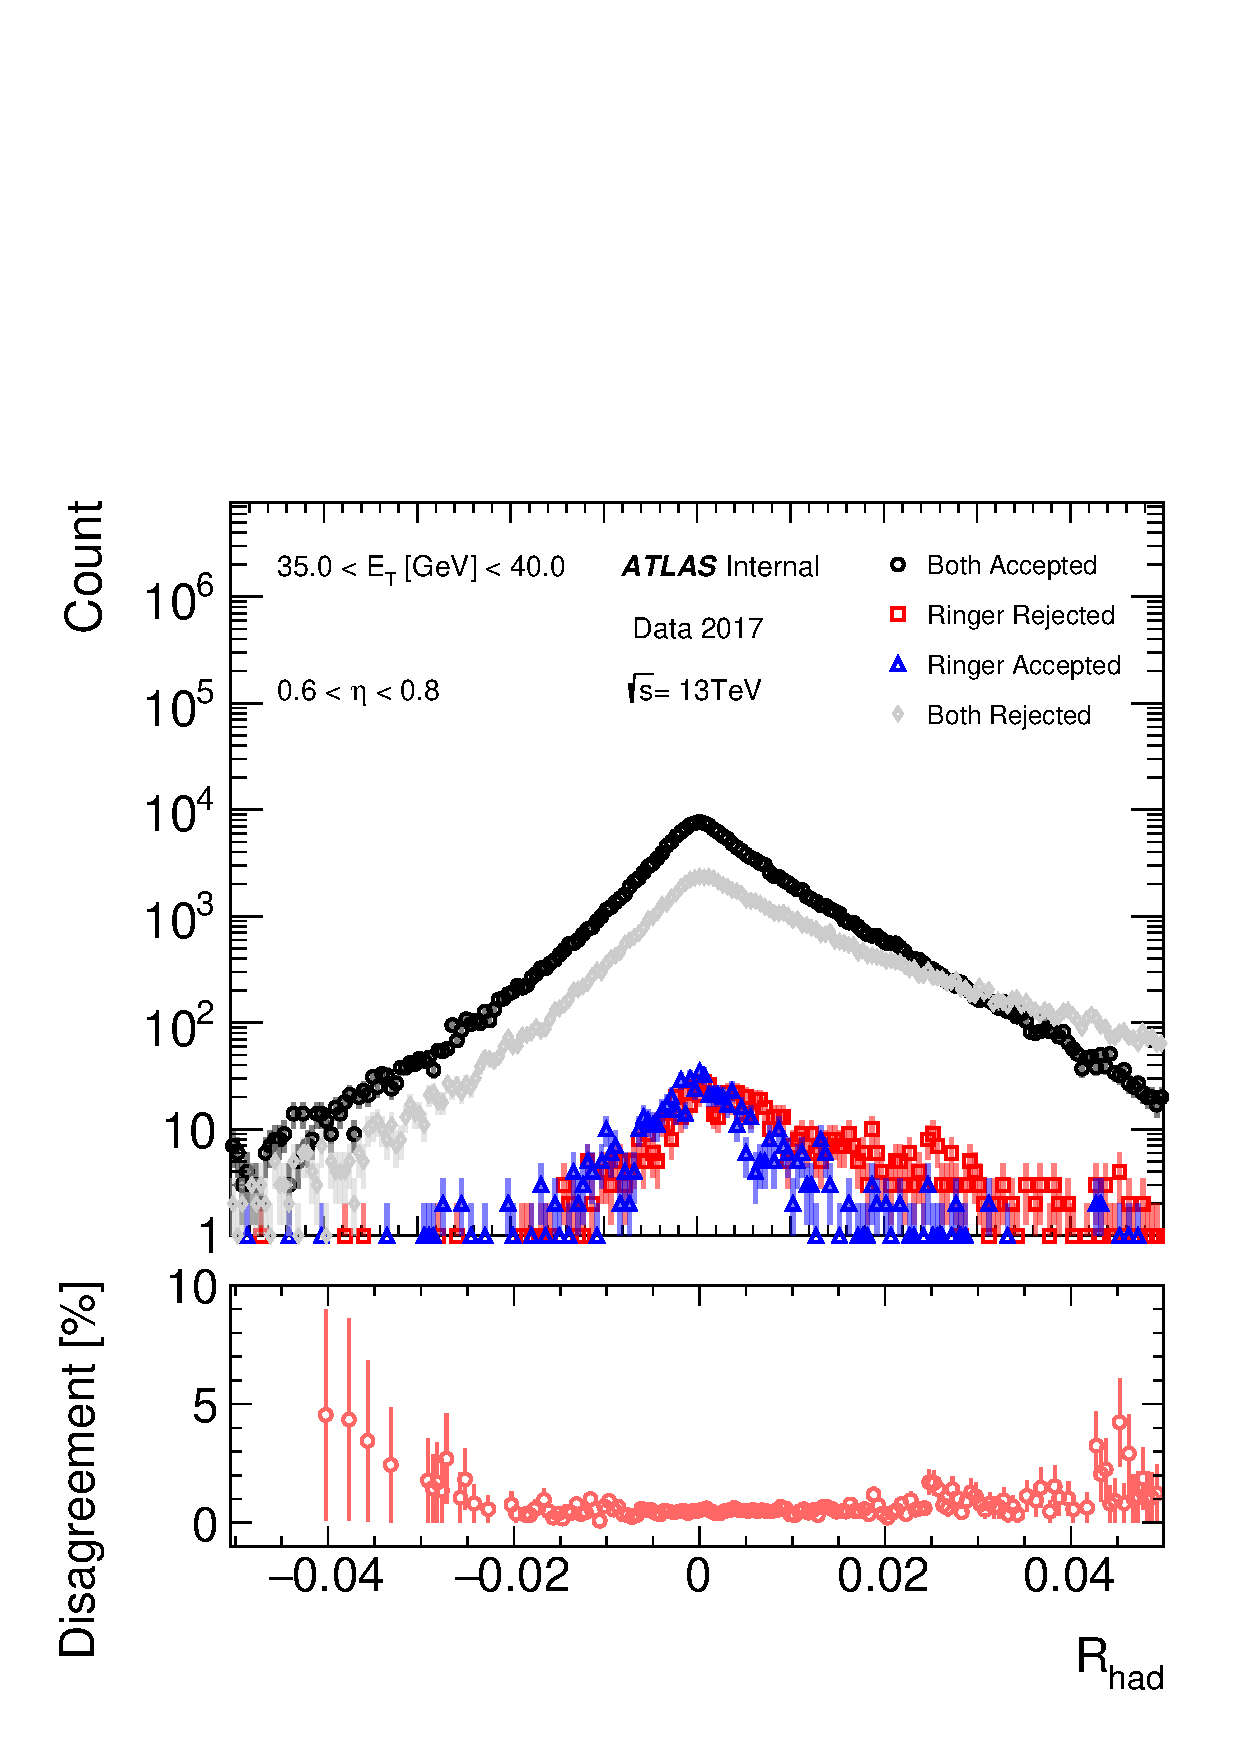
\includegraphics[width=\textwidth]{sections/05_analysis/figures/quadrant_plots/rhad.pdf}
\caption{}
\end{subfigure} \\


\caption{\label{fig:quadrant_calo_variables_30GeV}
    Quadrant Analysis plots for a selection of shower-shape variables used in the offline electron identification algorithm for the $0.6<\abseta{}<0.8$ and $30<\et{}<35$~\GeV region. The top pad in each figure shows the raw number of candidates for the four mutually exclusive cases: accepted both with and without 
	the \rnn{} (black); accepted only with the \rnn{} (blue); accepted only without the \rnn{} (red); rejected both with and without the \rnn{} (grey). The bottom pad shows 
	the disagreement as defined in Eq.~\eqref{eq:disagreement}.
}
%Quadrant analysis plots for the offline-reconstructed
%calorimetry variables employed in the
%likelihood and \wstot{} for the $0.6<\abseta{}<0.8$ and
%$30<\et{}~[\text{GeV}]<40$ slices.}%
\end{figure}


\begin{comment}
    
\begin{figure}[h!tb]
%\centering
%\begin{subfigure}[c]{.49\textwidth}
\centering
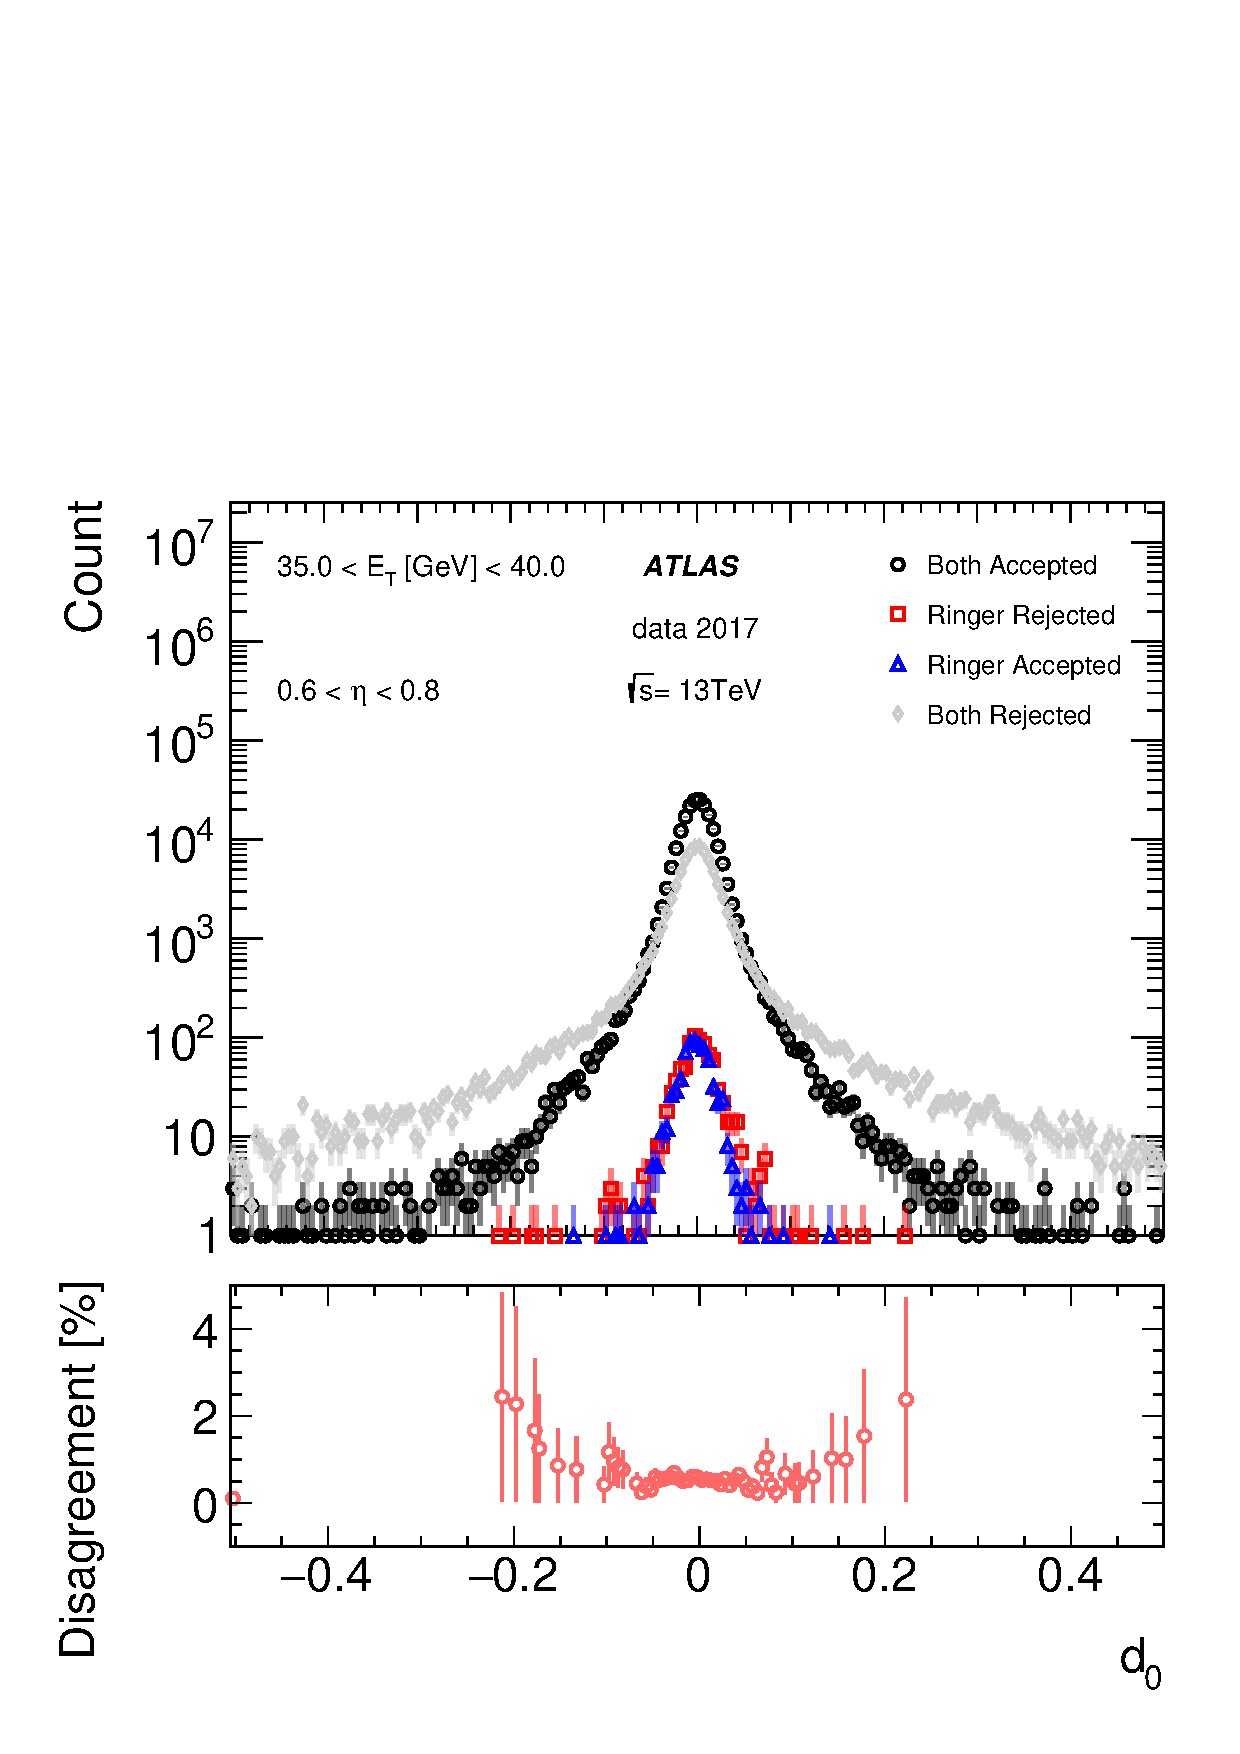
\includegraphics[width=.5\textwidth]{sections/05_analysis/figures/quadrant_plots/d0.pdf}
\caption{\label{fig:quadrant_track_variables_30GeV}
Quadrant analyses plots for the offline-reconstructed ID variable $d_0$ employed in the
likelihood for the $0.6<\abseta{}<0.8$ and $35<\et{}~[\text{GeV}]<40$ slice. The variable $d_0$ is defined as the transverse parameter of the impact point with respect to the collision beam.
}
\end{figure}
\end{comment}






\FloatBarrier
\subsection[Homogeneity Tests]{Homogeneity Tests}\label{ssec:agreement}

In this analysis, the impact on the offline likelihood identification requirements of using different triggers, \rnn{} and cut-based, applied either to the tag electron, is evaluated. 
This study requires a pair of duplicated triggers, applying a HLT\_e28\_lhtight\_nod0\_(noringer)\_ivarloose trigger selection with and without the \rnn{} (noringer), operating together online. The analysis is performed using the full 2027 collision data with the same selection as used for the offline likelihood optimization for electrons with \ET above \SI{15}{\GeV}~\cite{PERF-2017-01}.






%To benefit from the full 2017 dataset, collision data collected before TS1 were also employed. If the profiles of the calorimetry and track variables are statistically identical, the \rnn{} trigger is not expected to cause any relevant change in the derivation of the offline likelihood PDFs.  
%The statistical method for profile evaluation is described in Section~\ref{top:homogeneity_method} and the results are available in Section~\ref{top:agreement_homogeneity_results}.




%\subsubsection{Method}\label{top:homogeneity_method}



The problem is addressed by applying homogeneity tests to histograms~\cite{homogeneity_test} in order to check for systematic effects of the trigger configuration. These tests are based on a test originally developed by Pearson~\cite{pearson1911probability} and popularly employed in many fields beyond high-energy physics, e.g.\ social sciences~\cite{wickens2014multiway} and health~\cite{ma2015homogeneity}, where they are usually called contingency or consistency tests.

In order to benefit from the tests without having to customize them to an ATLAS-specific analysis set-up, the collision data were split into two
statistically independent groups or samples, consisting of data alternately taken from consecutive short time periods to keep their data-taking conditions as
similar as possible. 

The $p$-value, or probability value, is a measure used in statistical hypothesis testing to determine the significance of one's results. It represents the probability of obtaining an observed result if the null hypothesis (which states that there is no effect or no difference between the two trigger strategies) is true. By comparing the $p$-values of the two groups, it is possible to evaluate how the different configurations affect the likelihood that the profiles are being drawn from the same distribution. 
%If the $p$-values have negligible fluctuations with respect to the values obtained from tests comparing the same triggers, then the systematic effect in the profiles is negligible for a dataset that is half\footnote{Each group contains approximately half of the integrated luminosity.} of the size of the whole available dataset.

%\footnote{The p-value here is defined by: $P-value \approx f(x, k) = \frac{1}{2^{k/2}\Gamma(k/2)}x^{k/2 -1}e^{-x/2}$, where $x\in(0, \infty)$ and $k>0$}

To provide better insight into possible distortions, the corresponding 
individual $\chi_{i,j}^{s}$ contributions, allowing them to assume positive or negative values by defining

\begin{equation}
  \chi_{i,j}^{s} = \frac{(r_{i,j} - b_{i,j})}{\sqrt{b_{i,j}}},
  \label{eq:signed_chi}
\end{equation}

\noindent where $r_{i,j}$ ($b_{i,j}$) is the number of observations collected by the trigger with (without) the \rnn{} in $j^\text{th}$ histogram bin and in the $i^\text{th}$ $\et{}\times\abseta{}$ region.


\subsubsection{Results}\label{top:agreement_homogeneity_results}




Regardless the trigger configuration, the homogeneity tests between the two groups result in similar $p$-values. In other words, the fluctuations in the profiles are mainly statistical, with no sign of systematic effects due to the trigger configuration. 

Figure~\ref{fig:groups_homogeneity_calo} shows the residuals (bottom) for the \reta, \rphi, \eratio, and \rhad  calorimetry variables when the reference histogram is obtained from collision data collected by the trigger without the \rnn{} for the first group (top). The residuals are dominated by statistical fluctuations (i.s., the residual values fluctuate around a central value), and are within the expectations from the homogeneity hypothesis for most variables and regions. Similar behavior is observed for track variables. 

\begin{figure}[h!]
\begin{center}
\begin{subfigure}[c]{.48\textwidth}
\centering
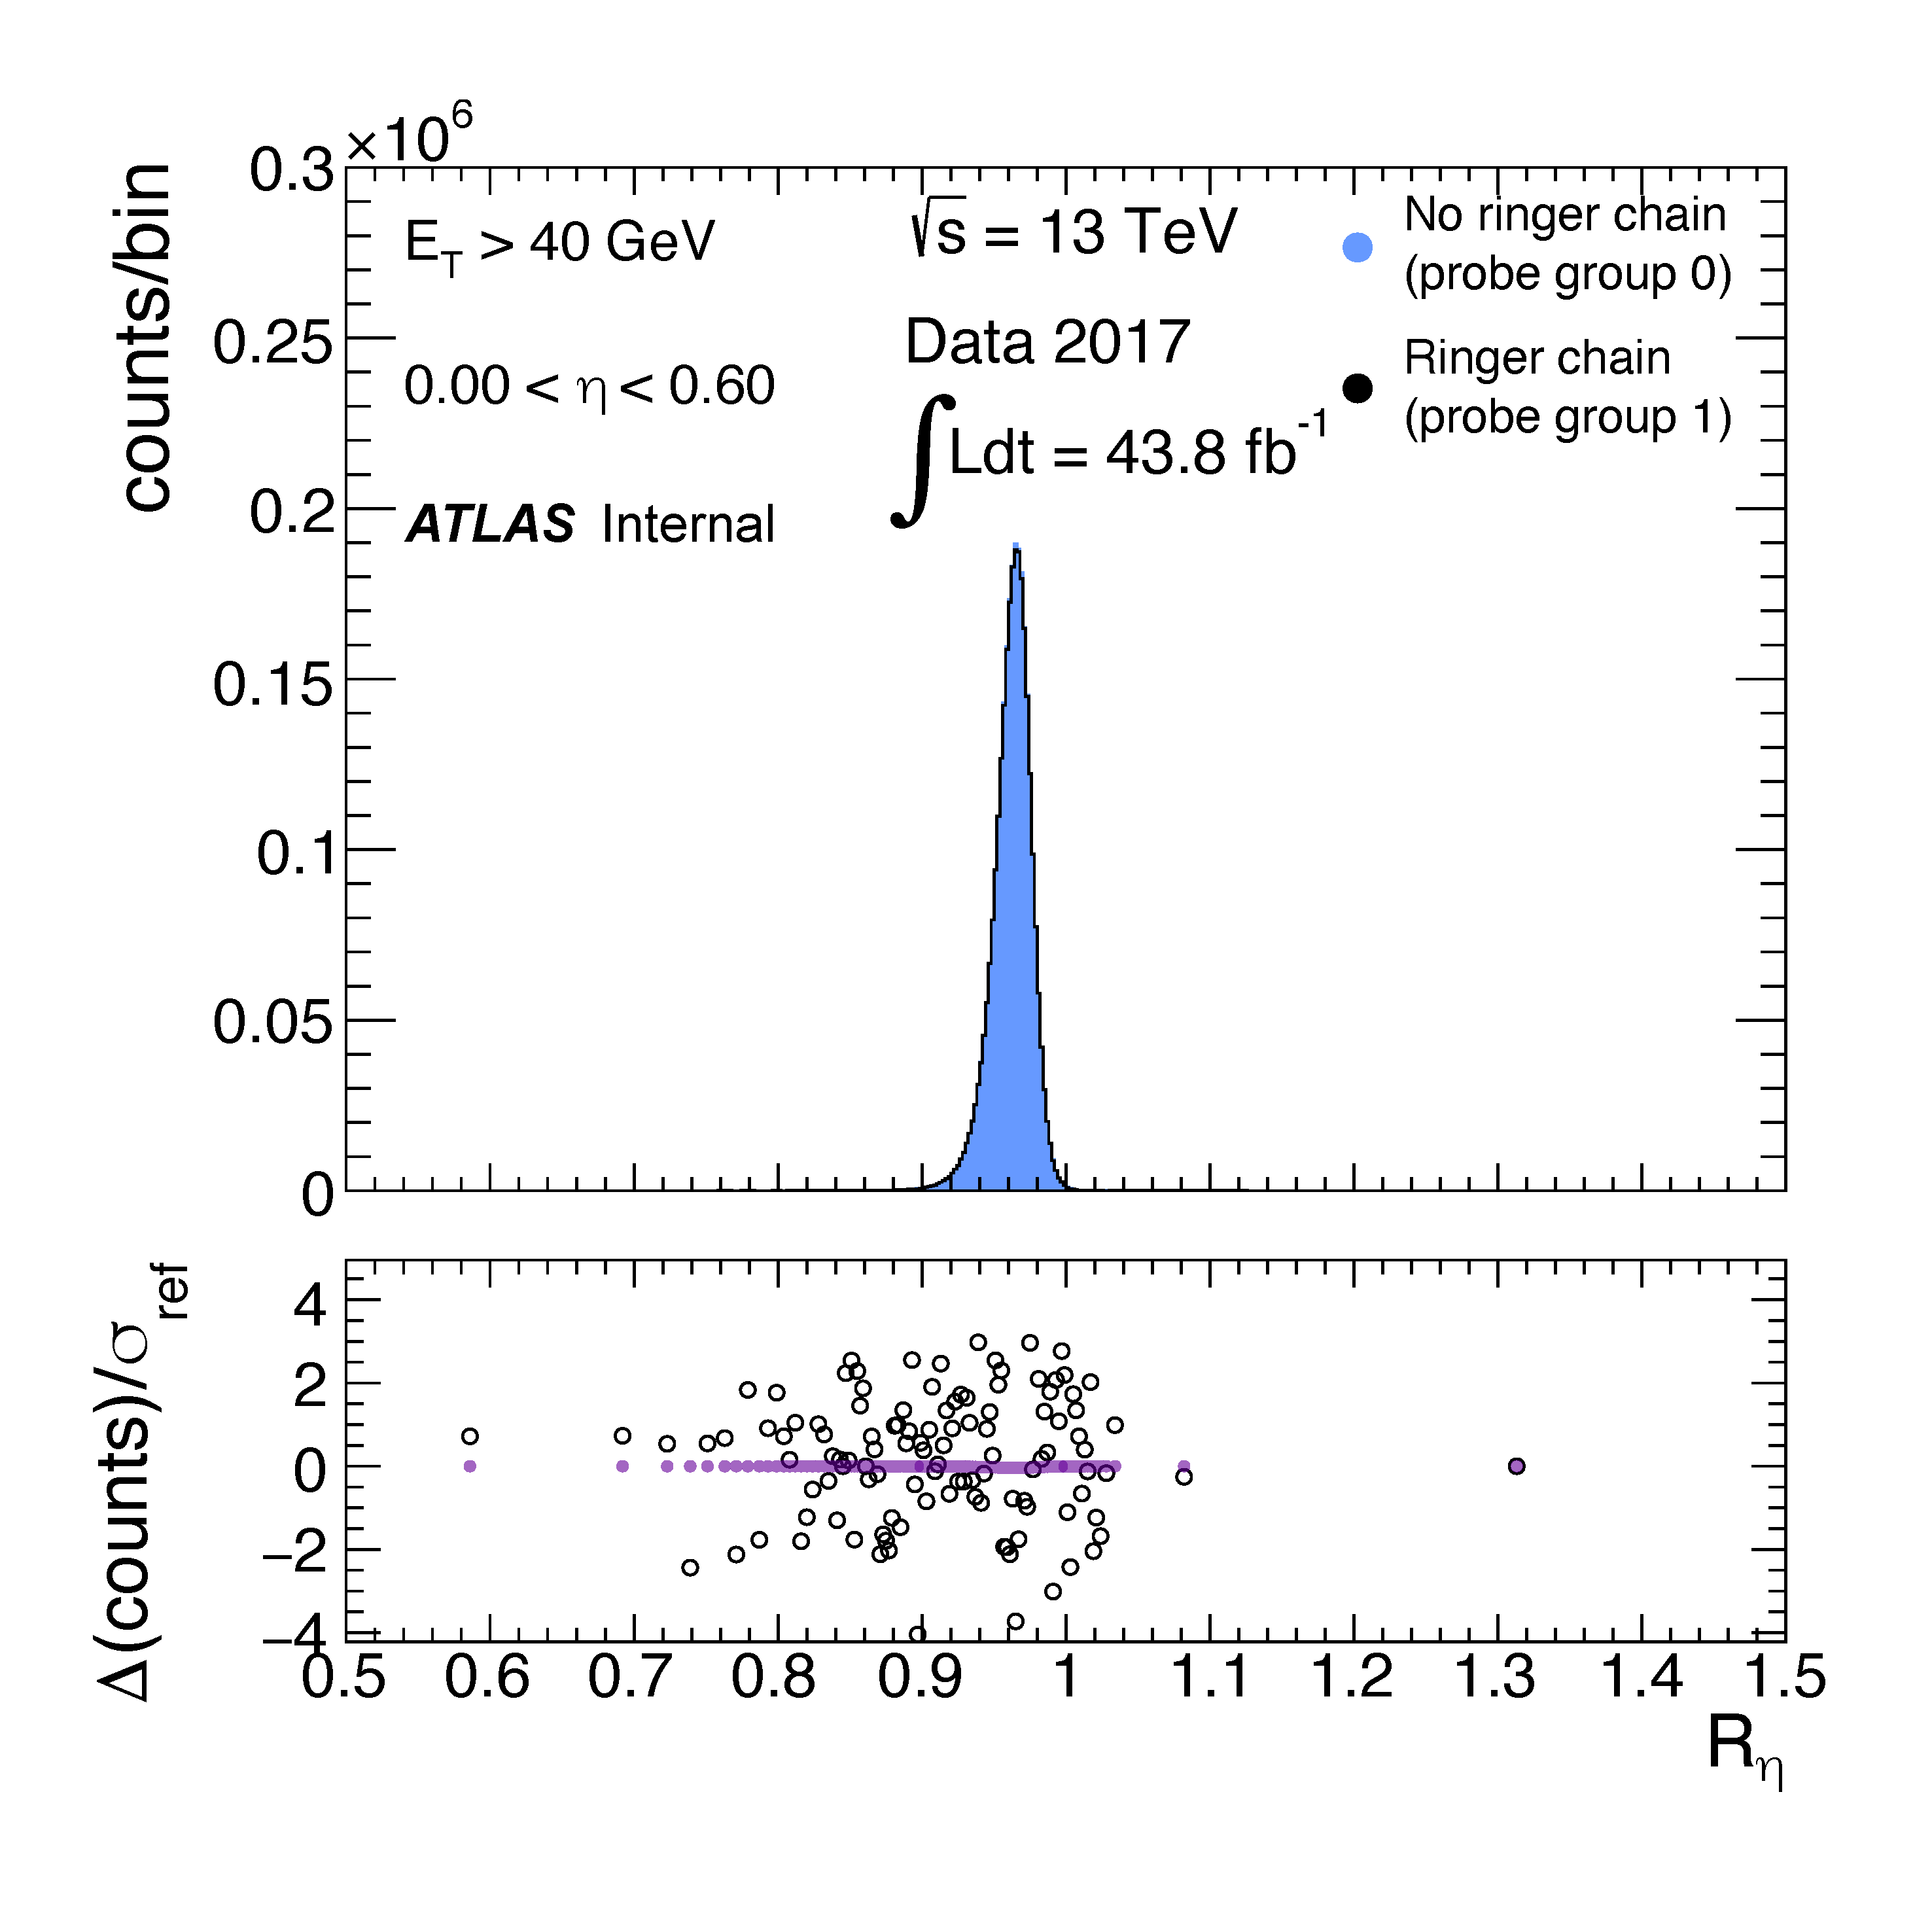
\includegraphics[width=\textwidth]{sections/05_analysis/figures/noAdjustment/el_reta_et40eta0_00_sigma_base_new.pdf}
\caption{}%

\end{subfigure}
\hfill
\begin{subfigure}[c]{.48\textwidth}
\centering
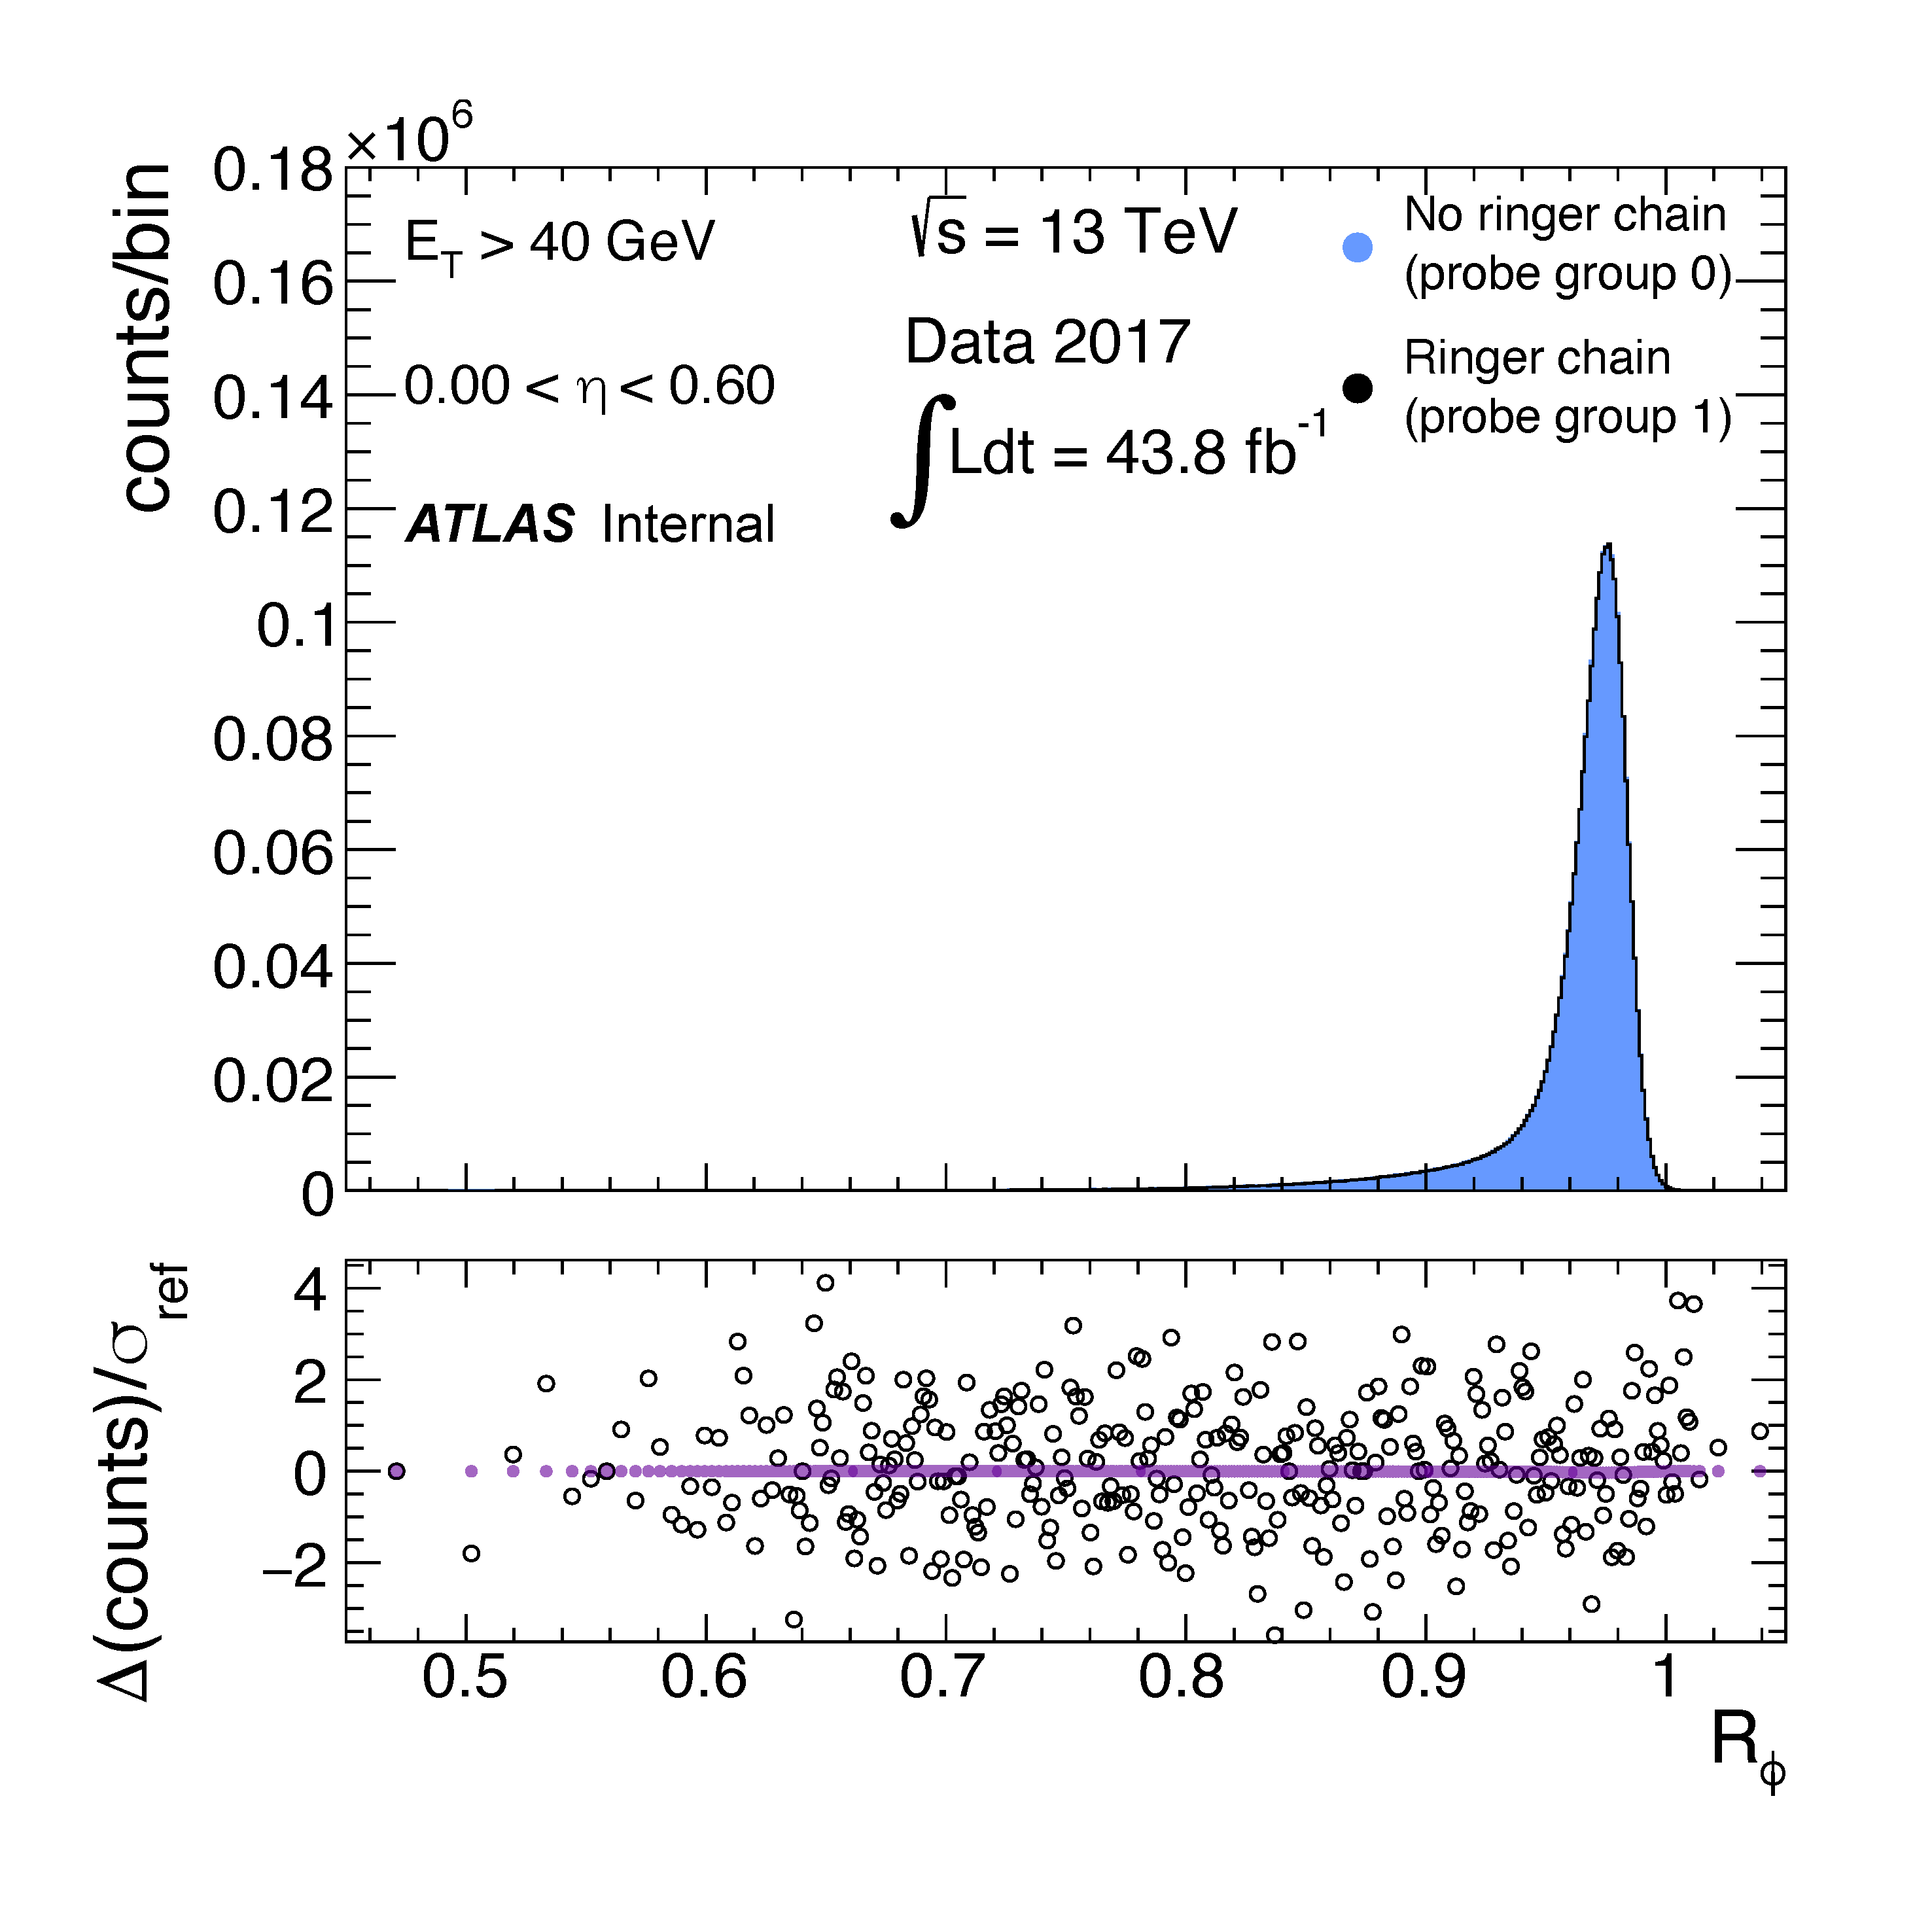
\includegraphics[width=\textwidth]{sections/05_analysis/figures/noAdjustment/el_rphi_et40eta0_00_sigma_base_new.pdf}
\caption{}%

\end{subfigure} \\
\begin{subfigure}[c]{.48\textwidth}
\centering
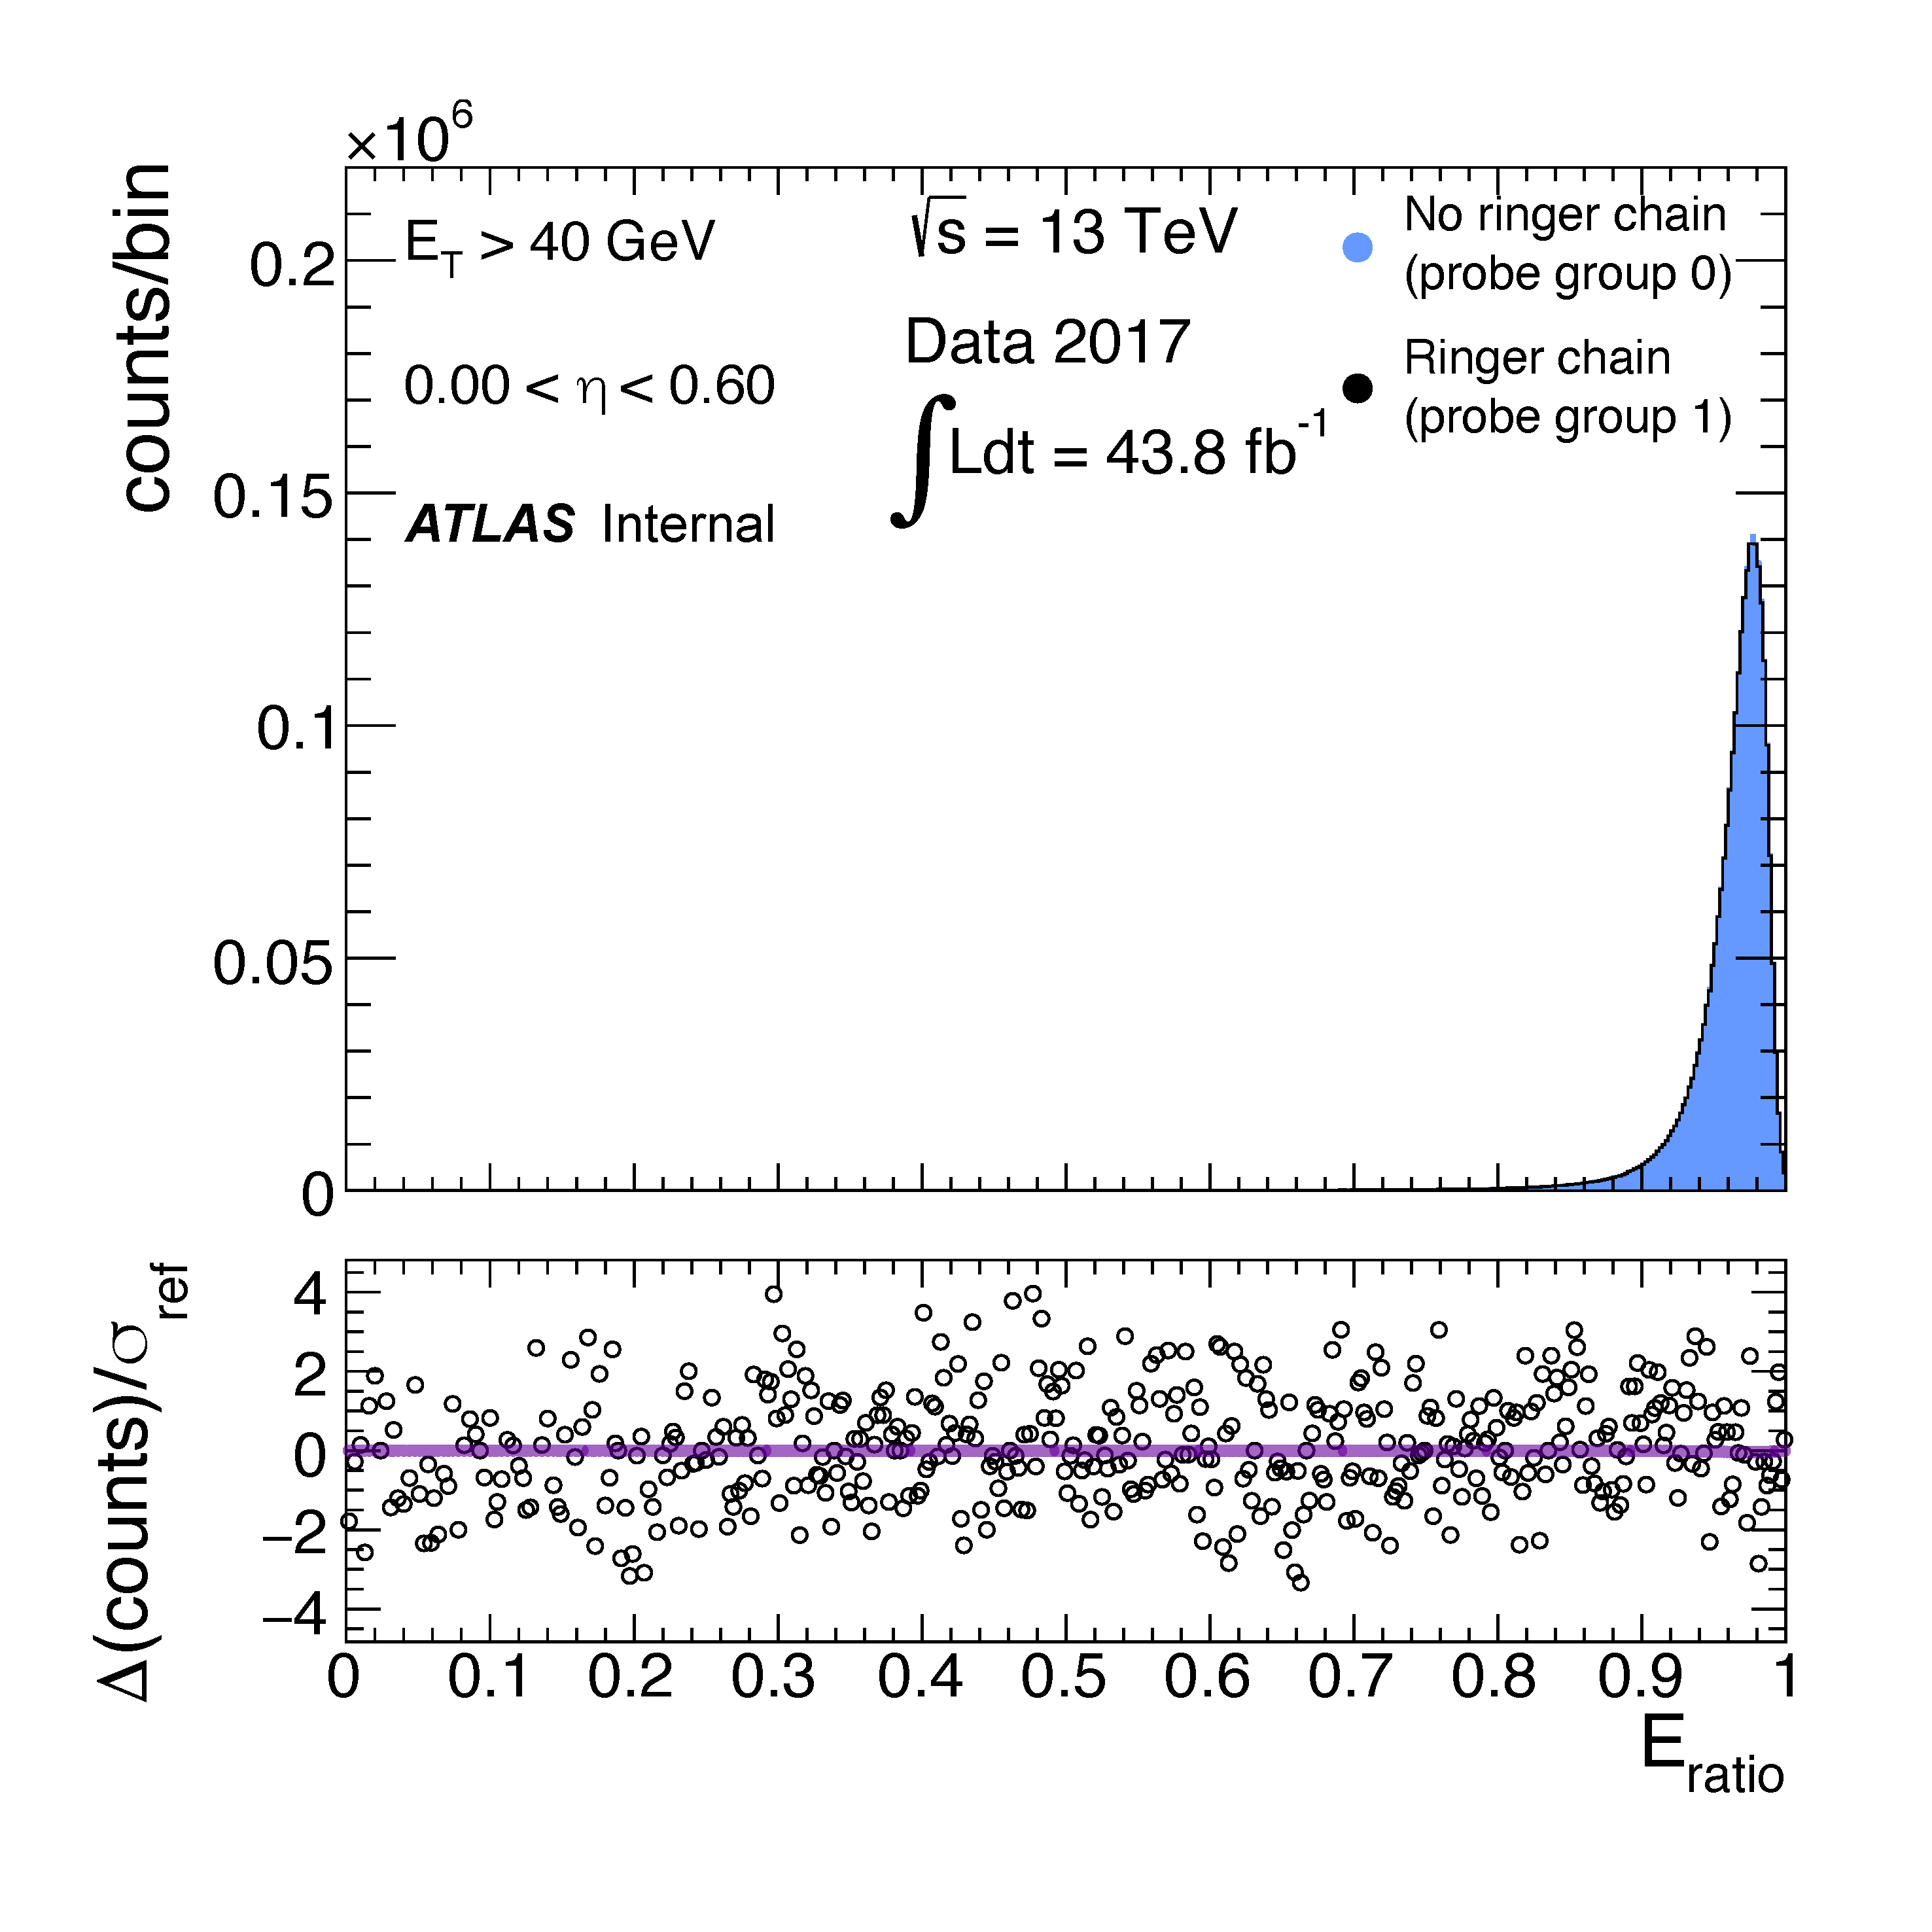
\includegraphics[width=\textwidth]{sections/05_analysis/figures/noAdjustment/el_eratio_et40eta0_00_sigma_base_new.pdf}
\caption{}%

\end{subfigure}
\hfill
\begin{subfigure}[c]{.48\textwidth}
\centering
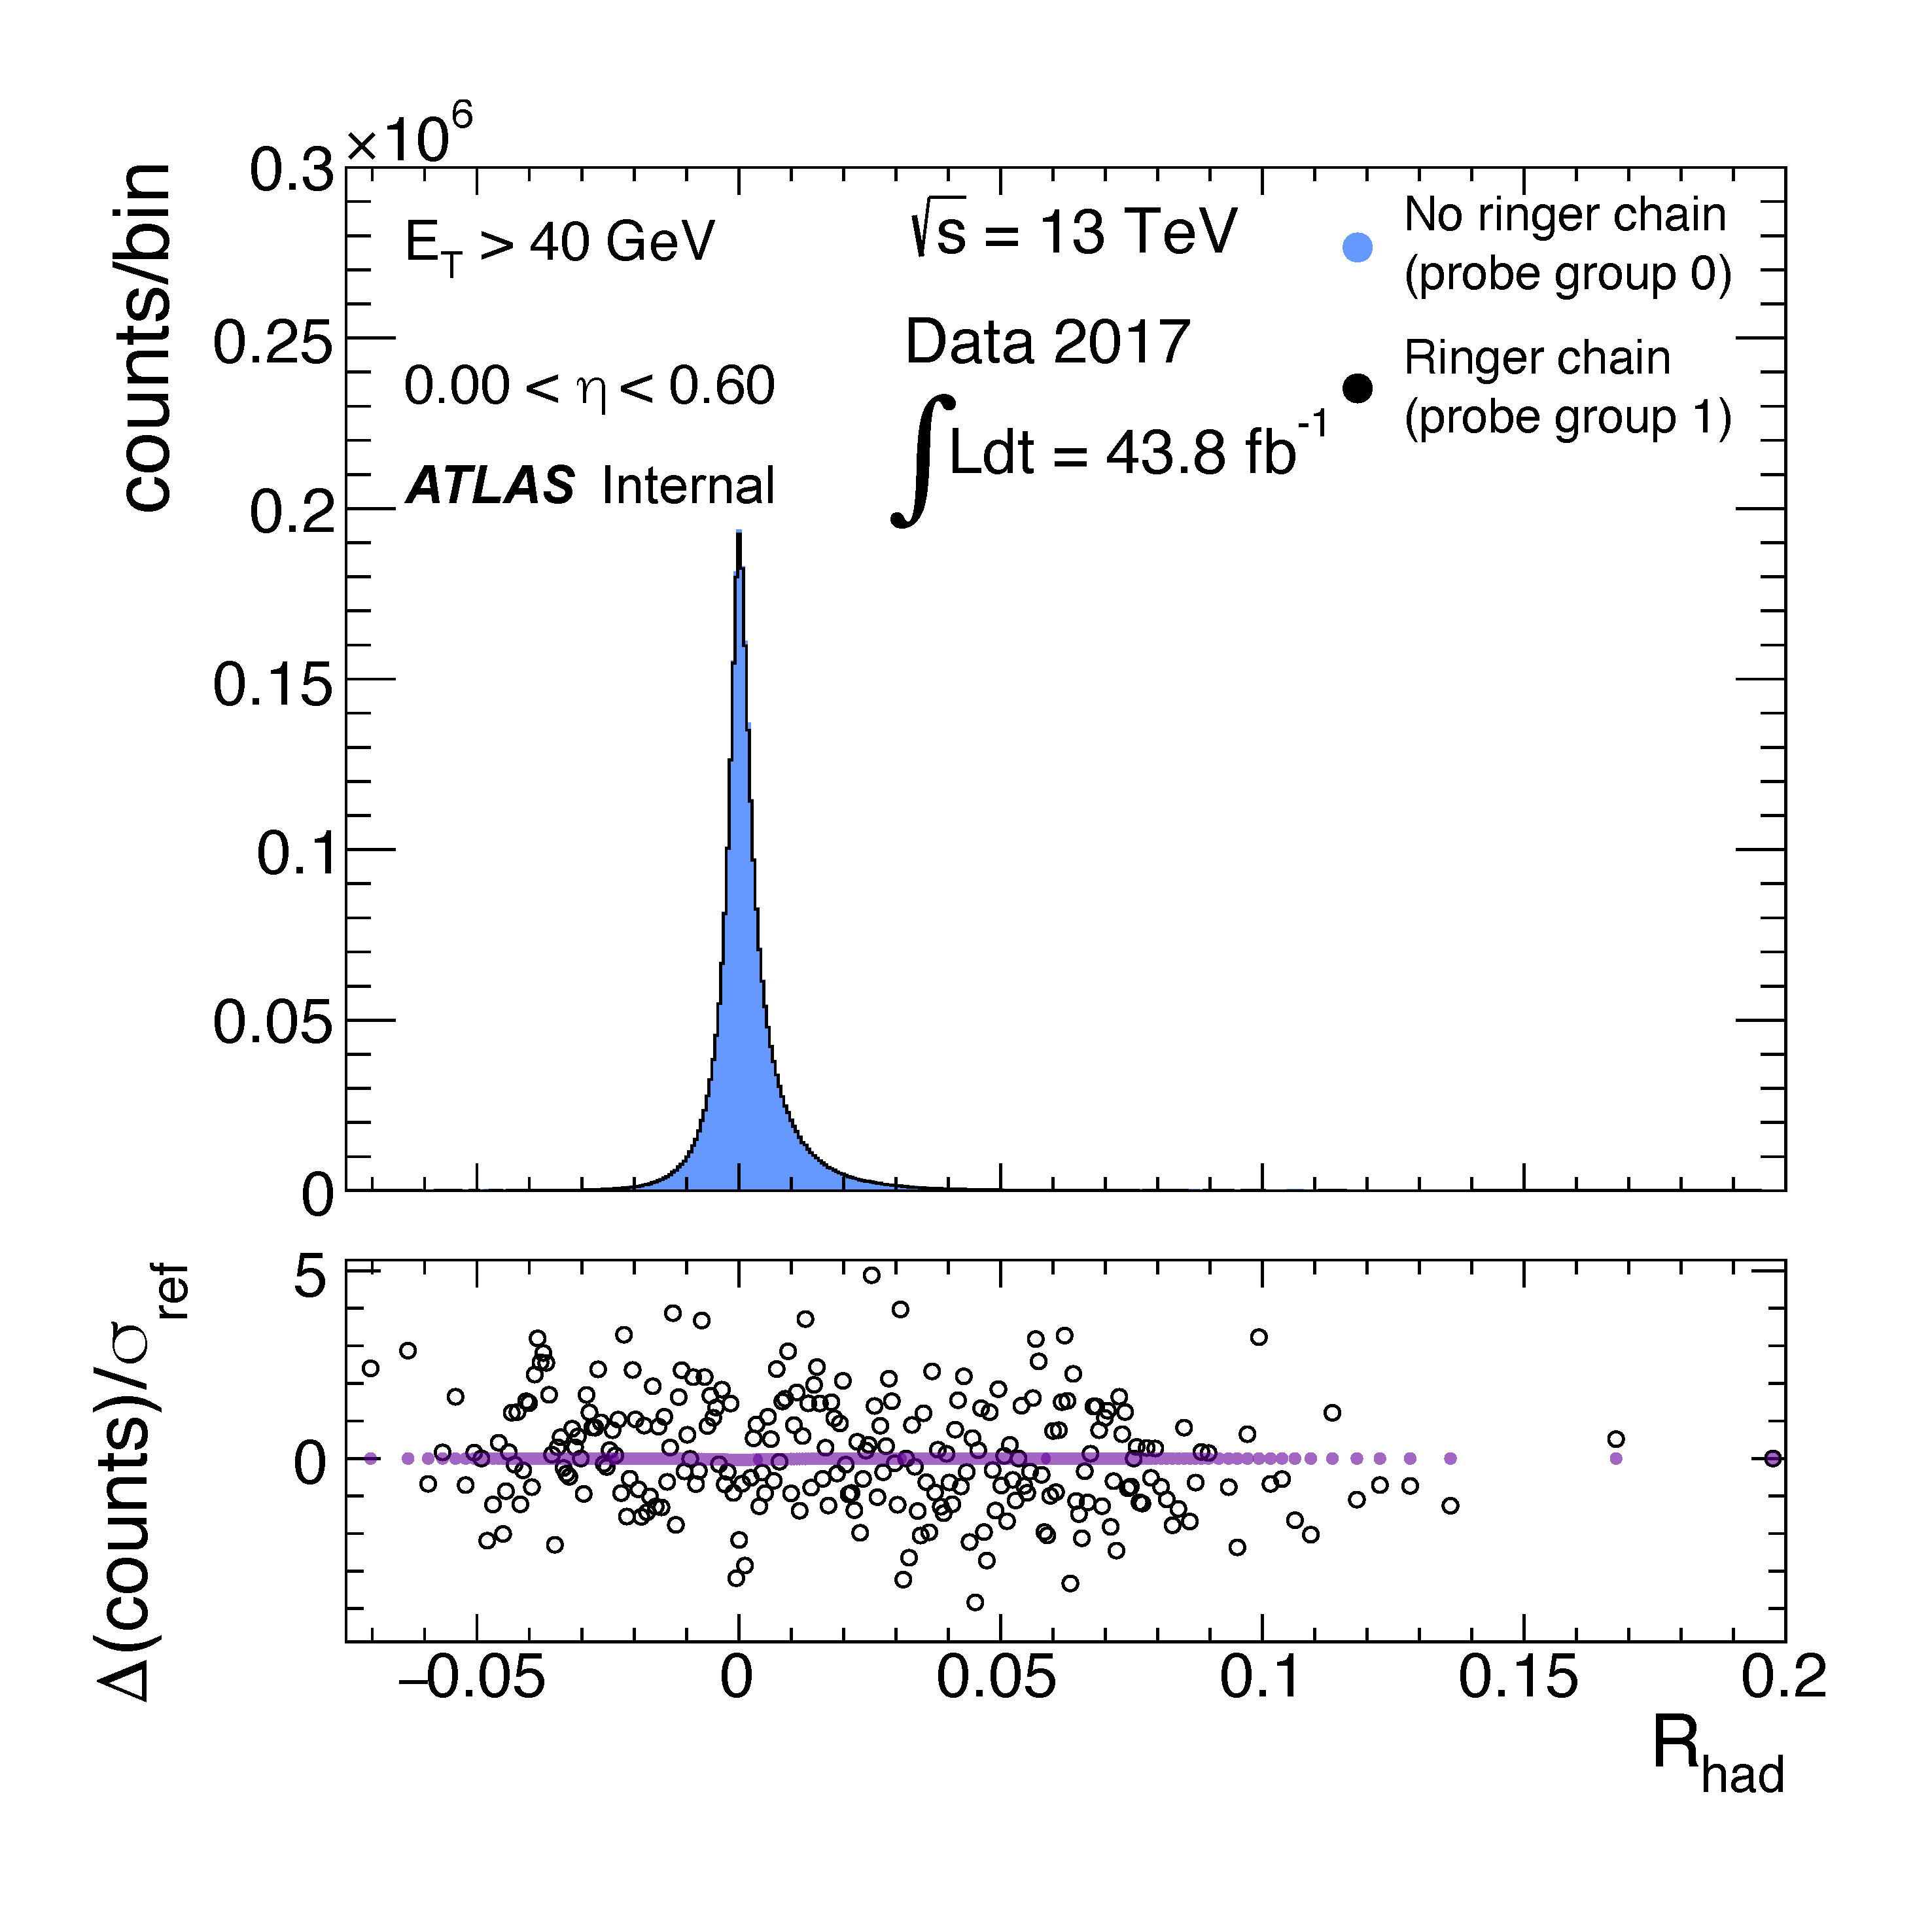
\includegraphics[width=\textwidth]{sections/05_analysis/figures/noAdjustment/el_rhad_et40eta0_00_sigma_base_new.pdf}
\caption{}%

\end{subfigure} \\
\caption{%
	Top: Profile histograms for the \reta, \rphi, \eratio, and \rhad calorimetry variables employed 
	in the offline likelihood in the $\et>\SI{40}{\GeV}$ and $0.0<\abseta{}<0.8$ regions using 
	collision data collected by triggering without the \rnn{} in the first arbitrary data group
	(blue area histogram) and collision data collected by triggering with the \rnn{} in the second
	arbitrary data group (black line histogram).  Bottom: residual contributions using 
	the $\chi^s$ statistic (black circles, from Eq.~(\ref{eq:signed_chi})), and the expected
	$\chi^s$ residuals if there are no distortions or statistical fluctuations with respect to the
	reference (purple dots at zero).
}%
\label{fig:groups_homogeneity_calo}
\end{center}
\end{figure}%


\FloatBarrier
